% Task-19 appendix: ManiGuard Jar history, protocol, search, confirmation details and integrity.
% Numbers come from progress/receipts/19-evo-adapter-results.md, configs/evo19/protocol.json,
% outputs/evo19/search/state.json and outputs/evo19/analysis/{summary,mechanism,revalidation}.json.
\section{ManiGuard Jar Details}\label{app:jar}
\subsection{Earlier Jar studies}\label{app:jar-history}
Task 19 is the latest of several attempts to help the same frozen policy on
Jar. The policy is ManiGuard's released Jar fine-tune of
$\pi_{0.5}$~\cite{black2025pi05,peng2026maniguard}, running in the
OmniGibson simulator of BEHAVIOR-1K~\cite{li2023behavior1k}. The baseline
replication (task 1) ran all 26 Jar scenes (ManiGuard numbers them as tasks;
we say scenes to keep ``task'' for our study numbers) with 20 Hz control, eight executed
targets per 16-target chunk, $256\times256$ cameras, a 2,000-step horizon and a
ten-step goal hold. It recorded 24 safe successes, seven unsafe successes, 37
safe failures and 36 unsafe failures in 104 attempts, with 43 counted violations and 103 engaged attempts. The
benchmark counts a violation only after first contact; a raw violation, used
from task 5 on, is any rule broken at any step. Of the 24 safe successes, 23 also closed
the jar before lifting it. Of the 43 violations, 33 were tips, eight lifted
the jar before closure and two did both at once.

Figure~\ref{fig:jar-history} places each later intervention beside the native
arm of its own study. The studies use different seeds, scenes and hosts, so
they are never pooled. A retreat triggered when the arm stopped moving (task 3) changed
neither safe success nor violations. An execution adapter with joint feedback
(task 5) and latent steering in the style of DSRL (task 7) did not help.
Slower joint targets passed a 12-attempt screen, 6/12 against 4/12, but not
their fresh-seed confirmation, 2/12 against 2/12 (task 8). The task 15 screen
favoured speed projection, 9/16 against 5/16 strict safe completions, but a
one-sided Fisher test gives $p=0.14$, and choosing among thirty-two sampled chunks reached only 3/16 or 4/16. Its confirmation lost two rented hosts and was never
completed; a partial mirror of it could not be verified and is not used here.
Task 15 also replayed stored observations: of 254 executed chunks recorded in
task 7 that failed a 0.10 m/s check (85 of them from the native arm), 122 had
a passing alternative among sixteen fresh policy samples. The speed-limit
stages of task 19 did not reproduce the screen's gain
(Section~\ref{sec:jar}). Task 3 counts benchmark safe success, which does
not require closing the jar first; the other rows use strict safe completion.

\begin{figure*}[t]
\centering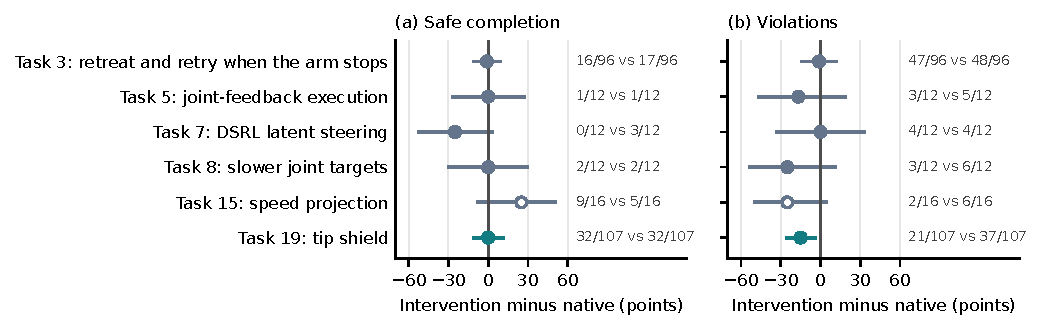
\includegraphics[width=\textwidth]{jar-history.pdf}
\caption{Every completed numbered Jar intervention study since the task 1
replication, plus the task 15 development screen, each against the native
policy in the same study, never pooled; earlier archived pilots are not shown. Dots are differences in percentage
points; lines are 95\% Newcombe intervals for two independent proportions,
which ignore pairing. The hollow marker is a development screen. Counts are
intervention versus native. Task 3 uses benchmark safe success and counted
violations; the others use strict safe completion and raw violations. Only
the task 19 violation interval excludes zero.}
\label{fig:jar-history}
\Description{A dot-and-interval chart with six studies. Safe completion
differences all have intervals spanning zero. For violations, only the task 19
tip shield has an interval entirely below zero.}
\end{figure*}

\subsection{Task 19 protocol}
The policy is the $\pi_{0.5}$ Jar checkpoint 7400, unchanged, served with
ManiGuard's evaluator at commit 6bf4c61 and its Jar configuration: 20 Hz joint
control, eight executed targets per 16-target chunk, $256\times256$ cameras, a
2,000-control horizon and a ten-step goal hold. The protocol was frozen at
22:10 UTC on 26 October 2026, before any search attempt. Its primary endpoint
is strict safe completion, evolved adapter minus native (the shield after
amendment 3), by a one-sided Fisher exact
test with Wilson intervals. Raw violation attempts were listed as a secondary
endpoint. Search attempts are training data, not effect estimates, and no
result is pooled with earlier Jar studies.

The search ran four stages, each with pycma~\cite{hansen2019pycma} in unit
coordinates, starting at the centre of the box with step size 0.25 (0.2 in
stage 2). Stage 1 evolved a near-jar speed projection with three genes: a speed
limit (0.03 to 0.30 m/s, log scale), a near radius (0.10 to 0.35 m) and a weight
for steps that move away from the jar (0 to 1). It tested eight candidates per
generation and scored four points for a strict safe completion, two for no
violation and one for grasping the jar. Stage 2 fixed the weight at one and
dropped the violation term. Stages 3 and 4 evolved the tip shield: tilt limit
$3+12u_0$ degrees and retreat distance $0.02+0.10u_1$ m, scored as four points
for a strict safe completion plus one point for no violation. Stages 2 to 4
tested six candidates per generation. Stage 3 counted contact only at the query control; stage 4
counted it over the eight controls up to the query, because the contact count
flickers during a push. Candidate $i$ of stage 4 generation $g$ ran scene $(0,3,6,9)_{i \bmod 4}$ with seed $195000+10g+i$. After eight generations the
distribution mean was frozen as the shield.

\begin{table*}[t]
\caption{Task 19 protocol amendments, all times UTC on 26 and 27 October 2026.
The last column states which confirmation outcomes existed when each change was
recorded, by host finish time; the dated records list 17 native outcomes as
visible at amendment 2 and 60 shielded at amendment 7. No amendment re-scored a finished attempt or changed the primary endpoint;
amendments 2 to 4 changed the search, its score and with it the adapter the
evolved arm would deploy (the shield from amendment 3), and amendments 3 and
4 redefined the optional hand-set arm that amendment 6 cancelled.}
\label{tab:jar-amendments}\centering\small
\begin{tabularx}{\textwidth}{rlXl}
\toprule
& Time & Change & Confirmation attempts finished \\
\midrule
1 & 22:37 & Confirmation panel enlarged from 48 to 72 pairs (seeds 193000--193017), interleaved in seed order; the optional hand-set speed-limit arm scheduled after both primary arms & 0 native, 0 shield \\
2 & 23:35 & Stage 1 closed as exploratory; stage 2 fixes the retreat weight at one & 18 native, 0 shield \\
3 & 23:51 & Stage 2 closed as exploratory; stage 3 evolves the tip shield & 21 native, 0 shield \\
4 & 23:59 & Stage 3 closed as a pilot; stage 4 counts contact over eight controls & 22 native, 0 shield \\
5 & 00:00 & Exact tests fixed for the listed violation endpoint (Fisher, Barnard, exact McNemar) & 22 native, 0 shield \\
6 & 01:07 & Hand-set arm cancelled; panel extended by seeds 193018--193029 to 120 pairs & 47 native, 0 shield \\
7 & 01:48 & Scheduling only: remaining jobs run in pair order so a time cut leaves complete pairs & 48 native, 62 shield \\
\bottomrule
\end{tabularx}
\end{table*}

\begin{figure*}[t]
\centering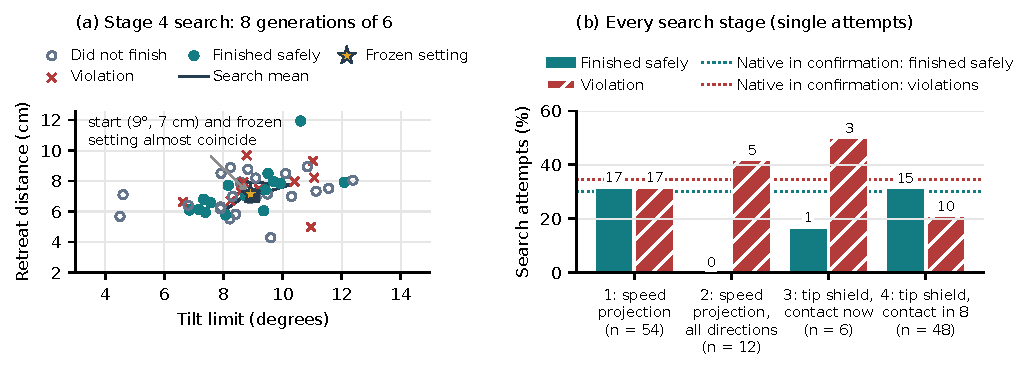
\includegraphics[width=\textwidth]{evo19-search.pdf}
\caption{The task 19 search. (a) Every stage 4 candidate, coloured by its single
attempt's outcome, with the path of the CMA-ES mean. The mean ended close to its
hand-chosen start. (b) Outcomes of each search stage. The dotted lines mark the
native policy's rates in confirmation, which used different seeds; search
attempts are training data, not effect estimates.}
\label{fig:jar-search}
\Description{Left: a scatter of 48 candidate settings around 9 degrees and 7 cm
with the search mean wandering near its start. Right: bars of safe completion and
violation rates for the four search stages.}
\end{figure*}

\subsection{Confirmation details}\label{app:jar-confirm}
Table~\ref{tab:jar-detail} breaks the confirmation down by scene and by
outcome. Scene 9 is the hardest for both arms. The rule-replay columns
apply the frozen trigger to each recording: at a policy query before any
violation, tilt at least 8.92 degrees and robot contact in the last eight
controls. For the shield arm the replay fires in exactly the 50 attempts that logged a
retreat (255 retreat chunks in all, each also reproduced by the per-decision
replay in the integrity checks). For the native arm it marks where the shield
would first have acted; after that point the two arms would diverge, so it
is not a prediction of the shielded outcome. Violations happen before the jar
is closed in 11 native and 7 shielded attempts, and after closure in 26 and 14.

\paragraph{Intervals and endpoints.} Differences are shield minus native with
95\% Newcombe hybrid-score intervals~\cite{newcombe1998interval}, built
from Wilson score intervals~\cite{wilson1927probable}, which
match the unpaired Fisher and Barnard tests. Strict safe completion, the
primary endpoint, differs by 0.0 points, $[-12.1,12.1]$; violations differ by
$-15.0$ points, $[-26.3,-3.0]$. The protocol listed six secondary endpoints and fixed no multiplicity
correction; amendment 5 named raw violations the key secondary. Bonferroni
over the primary and that endpoint asks for $p<0.025$, which the violation
test meets (Fisher $p=0.010$, Barnard $p=0.008$); over all seven listed
endpoints it asks for $p<0.0071$, which it does not. The primary endpoint
shows no effect. The original 72-pair panel alone shows the same pattern, 25
against 13 violations and 22 against 25 strict safe completions. One shielded
attempt (scene 9, seed 193026) has no native partner because its native
attempt did not finish before the stop; it was a violation, and adding it gives 22/108.

\paragraph{Post hoc checks on timing.} The shield was designed at amendment 3
(23:51 UTC) and frozen at 01:07:13 UTC, 42 seconds before amendment 6 was
recorded, while native confirmation
attempts were already finishing (Table~\ref{tab:jar-amendments}). The violation test was fixed before any shielded attempt, but the design did
use native outcomes: amendment 3 records that five native confirmation violations were inspected
together with 17 search violations; by then 21 native attempts, seven of them
violations, had finished. Dropping the 21 pairs whose native
attempt finished before amendment 3 leaves 30/86 against 15/86 violations,
$-17.4$ points, $[-29.9,-4.3]$, one-sided Fisher $p=0.007$, with 22 against 23
strict safe completions. Dropping the 45 pairs whose native attempt finished
before the freeze leaves 20/62 against 12/62, $-12.9$ points, $[-27.6,2.5]$,
$p=0.075$, with 17 against 14 strict safe completions. Both keep the
direction; the second is not significant alone. These cuts are post hoc and
descriptive.

\paragraph{Outcome changes within pairs.} Table~\ref{tab:jar-transitions}
crosses each pair's native outcome with its shielded one. Because attempts
are not deterministic per seed, a cell is not a causal effect on that
scene. In 22 pairs the native attempt broke a rule and the shielded one did not, and
in six the reverse; 12 pairs combine a native safe completion with a shielded
stall, and 8 combine a native violation with a shielded safe completion.

\begin{table}[t]
\caption{Outcomes within the 107 matched pairs: rows native, columns shield.}
\label{tab:jar-transitions}\centering\small
\begin{tabular}{lrrrrr}
\toprule
Native $\downarrow$ / shield $\rightarrow$ & Safe & Viol. & Stall & Never & Total \\
\midrule
Strict safe & 15 & 3 & 12 & 2 & 32 \\
Violation & 8 & 15 & 11 & 3 & 37 \\
Stalled after closing & 6 & 0 & 14 & 6 & 26 \\
Never closed & 3 & 3 & 3 & 3 & 12 \\
\midrule
Total & 32 & 21 & 40 & 14 & 107 \\
\bottomrule
\end{tabular}
\end{table}

\begin{table}[t]
\caption{Jar confirmation by scene and by outcome; each N / S cell gives native /
shield. ``Rule
fires'' counts attempts in which the frozen trigger holds at a query before any
violation.}
\label{tab:jar-detail}\centering\small
\begin{tabular}{lrrr}
\toprule
By scene & Pairs & Strict safe (N / S) & Violations (N / S) \\
\midrule
Scene 0 & 27 & 14 / 9 & 9 / 7 \\
Scene 3 & 27 & 7 / 11 & 8 / 2 \\
Scene 6 & 27 & 10 / 10 & 7 / 4 \\
Scene 9 & 26 & 1 / 2 & 13 / 8 \\
\midrule
By outcome & & Attempts (N / S) & Rule fires (N / S) \\
\midrule
Strict safe & & 32 / 32 & 9 / 10 \\
Violation & & 37 / 21 & 34 / 17 \\
Stalled after closing & & 26 / 40 & 10 / 19 \\
Never closed & & 12 / 14 & 4 / 4 \\
\bottomrule
\end{tabular}
\end{table}

\subsection{Integrity, cost and preservation}
Each confirmation attempt was validated on its host from the recording and
the monitor's record, including an exact replay of every shield decision.
All 215 counted confirmation attempts were validated again on the workstation
and match both the stored records and the host checks. One worker ran a
shield job a second time straight after its counted attempt had finished. The
duplicate is excluded; it ended without finishing, so counting it instead
would lower the shield's strict safe count by one and change no violation
count. A deliberate repeat of one native attempt closed the jar and tipped
late, where the original tipped before closure, which shows that attempts are
not deterministic per seed. The run used eight single-GPU rentals (seven RTX
3090 and one RTX 4090, several replaced early when slow or failing) between
21:43 and 02:57 UTC, at a conservative estimated cost of US\$8.58. Every attempt
is preserved in the private dataset
\texttt{Sachioster/maniguard-jar-replication-20261022} under
\texttt{evo19/}, revision \texttt{98e8fe31}, with 5,564 files re-downloaded
and checked by SHA-256.
